\newpage 
\section{Part 4: CAN-Ethernet-Gateway on Infineon \\AURIX TC297}\label{sec:can-gateway}

This chapter focuses on the implementation of a CAN-Ethernet gateway.

\subsection{Aim of the Practical Work}
The objective of this work is to design, implement, and validate a bidirectional gateway that transparently links a classical CAN bus to a standard Ethernet network on an Infineon AURIX TriCore evaluation board. Requirements for the gateway are:
\begin{itemize}
\item \{CAN → Ethernet\}: listen on the CAN bus, encapsulate every accepted CAN frame in an IPv4/UDP (or alternatively RAW) payload, and forward it so that any IP-based device can interpret native CAN traffic
\item \{Ethernet → CAN\}: accept UDP or RAW Ethernet frames that carry a properly formatted CAN payload, reconstruct standard CAN data frames and re-inject them onto the bus with correct arbitration timing
\end{itemize}
This compact overview frames the subsequent sections, which will give details about the hardware, concept and system architecture. 
\subsection{Hardware Overview: Infineon AURIX TC297}
% Describe the microcontroller and its relevant peripherals.
The Infineon TriCore microcontroller combines the capabilities of a microprocessor, microcontroller, and digital signal processor into one integrated platform, making it highly suited for automotive applications demanding real-time responsiveness and robust processing power.\\\\
Built around three 32-bit TriCore TC1.6P CPUs that run at up to 300 MHz, it couples up to 8 MB of ECC-protected flash with 728 kB on-chip RAM and a 128-channel DMA engine on a low-latency SRI cross-bar, so firmware can move payloads without stalling the cores. Gateway-relevant peripherals are integrated on-chip: a MultiCAN+ module with six independent CAN-FD-capable nodes and 10/100 Mbit/s Ethernet MAC that connects to an external PHY through MII or RMII. Because both engines share the same system bus, frames can be moved between CAN and Ethernet within deterministic microsecond budgets. A hardware security module, lock-step safety core, and redundant timer blocks complete the feature set required for ISO 26262 ASIL-D designs, making the TC297 a compact single-chip platform for the real-time CAN–Ethernet gateway realised in this project\cite{infineon}.
% Mehr ins Detail gehen?

\subsection{Theoretical Concept }
A bidirectional gateway has to move information between two networks that sit at different layers of the ISO/OSI model: CAN is a controller-centric field bus defined entirely at layer 2, whereas Ethernet is normally used as the physical bearer for layer-3 protocols such as IPv4. The design therefore needs an encapsulation scheme that (i) preserves every CAN frame bit-exactly, (ii) introduces only constant and minimal latency, and (iii) passes unhindered through standard switching, routing and diagnostic equipment.\\\\
% Bitte schreiben wieso UDP und nicht RAW
A classical CAN data frame carries an 11- or 29-bit identifier, a data length code (0-8 bytes in CAN 2.0, up to 64 bytes in CAN FD), the data field itself, plus bus-internal CRC and ACK bits. When the frame is moved to Ethernet only the semantic content must be preserved; the physical-layer bits are regenerated by the MULTICAN+ controller on retransmission. The project therefore serialises every CAN frame as a fixed-length record inside the UDP payload: four bytes little-endian identifier, one byte DLC, eight data bytes zero-padded, followed by one control byte whose individual bits flag extended identifiers and RTR frames. A short ASCII “magic” header (“ISO11898”) and a version byte at the start of the datagram allow a receiver to detect mis-alignment. Up to sixteen such records share one datagram, which keeps Ethernet utilisation high.

\subsection{Software Implementation}
% Explain the software design and key algorithms.
The implementation starts with configuring the necessary hardware peripherals on the TriCore board, such as CAN and Ethernet modules. This is accomplished by using an initialization routine (Listing 1).
\begin{lstlisting}[language=C, caption={Initialization of modules (Cpu0\_Main.c)}, label={lst:ini_module}]
void initModules(void)
{
    /* Disable watchdog timers for stable operation */
    IfxScuWdt_disableCpuWatchdog(IfxScuWdt_getCpuWatchdogPassword());
    IfxScuWdt_disableSafetyWatchdog(IfxScuWdt_getSafetyWatchdogPassword());

    /* Initialize status LEDs for debugging */
    initAliveLed();
    initBlinkyLed();
    initTxSuccessLed();
    initBufferFailLed();
    initRXETHLed();

    /* Initialize communication interfaces */
    initMultican();
    initEthernet();

    /* Initialize timing functions */
    initBlinkyTimer();

    /* Initialize the gateway module */
    initGateway();
}
\end{lstlisting}
This initialization function disables watchdog timers to ensure uninterrupted operation and sets up peripherals necessary for the gateway’s functionality, such as LEDs for visual debugging and status indication. It initializes the Multican and Ethernet modules, sets up timing mechanisms for periodic tasks, and prepares the gateway functionality.\\\\
The gateway logic is executed periodically within the main execution loop through the function \verb|runGateway()|. This function orchestrates the two principal operations: the first function \verb|forwardCanToEthernet()| handles translating CAN messages to Ethernet packets. The converting of CAN messages into Ethernet frames is shown in Listing 2.
\begin{lstlisting}[language=C, caption={CAN to Ethernet message translation (Gateway.c)}, label={lst:can_to_eth}]
void forwardCanToEthernet(void)
{
    IfxMultican_Message rxMsg;
    /* Get a handle to the high-level CAN message object driver */
    IfxMultican_Can_MsgObj* rxMsgObjHandle = &g_multican.canRxMsgObj;

    /* Check if the dedicated RX message object has a new message */
    if (IfxMultican_Can_MsgObj_isRxPending(rxMsgObjHandle))
    {
        Ifx_CAN_MO* rxMo = IfxMultican_MsgObj_getPointer(g_multican.can.mcan, rxMsgObjHandle->msgObjId);

        IfxMultican_Can_MsgObj_readMessage(rxMsgObjHandle, &rxMsg);

        boolean isExtended = IfxMultican_MsgObj_isExtendedFrame(rxMo);
        boolean isRtr = FALSE;

        uint8 dlc = rxMsg.lengthCode;
        uint8 udpPayload[17];

        udpPayload[0] = 0x01;
        udpPayload[1] = 1;

        udpPayload[2] = (uint8)(rxMsg.id >> 0);
        udpPayload[3] = (uint8)(rxMsg.id >> 8);
        udpPayload[4] = (uint8)(rxMsg.id >> 16);
        udpPayload[5] = (uint8)(rxMsg.id >> 24);

        udpPayload[6] = isExtended;
        udpPayload[7] = isRtr;
        udpPayload[8] = dlc;

        uint8 can_data_bytes[8];
        can_data_bytes[0] = (uint8)(rxMsg.data[0] >> 0);
        can_data_bytes[1] = (uint8)(rxMsg.data[0] >> 8);
        can_data_bytes[2] = (uint8)(rxMsg.data[0] >> 16);
        can_data_bytes[3] = (uint8)(rxMsg.data[0] >> 24);
        can_data_bytes[4] = (uint8)(rxMsg.data[1] >> 0);
        can_data_bytes[5] = (uint8)(rxMsg.data[1] >> 8);
        can_data_bytes[6] = (uint8)(rxMsg.data[1] >> 16);
        can_data_bytes[7] = (uint8)(rxMsg.data[1] >> 24);

        for (int i = 0; i < dlc; i++)
        {
            udpPayload[9 + i] = can_data_bytes[i];
        }

        sendEthernetPacket(udpPayload, 9 + dlc);

        /*
         * FIX: Manually clear the Receive Pending flag.
         * This is the crucial step to prevent the same message from being read again.
         */
        IfxMultican_Can_MsgObj_clearRxPending(rxMsgObjHandle);
    }
}
\end{lstlisting}
When a CAN message is received, this function checks for pending messages, reads the data into a structured format, and encapsulates it into a UDP packet. Metadata including the CAN identifier, message length, and payload are meticulously formatted. This encapsulation is critical for ensuring accurate data representation over Ethernet and allows diagnostic and monitoring tools to interpret the data correctly.\\\\
The implementation of the second operation \verb|forwardEthernetToCan()|, that handles translating Ethernet packets to CAN messages, is implemented as shown in Listing 3.

 
\begin{lstlisting}[language=C, caption={Ethernet to CAN message translation (Gateway.c)}, label={lst:eth_to_can}]
void forwardEthernetToCan(void)
{
    uint8 ethPayload[17];
    uint16 payloadLen = receiveEthernetPacket(ethPayload, sizeof(ethPayload));

    if (payloadLen > 0)
    {
        // Packet validation
        if (payloadLen < 9 || ethPayload[0] != 0x01) { return; }
        uint8 dlc = ethPayload[8];
        if (dlc > 8 || payloadLen < (9 + dlc)) { return; }

        // Packet parsing
        uint32 can_id = ((uint32)ethPayload[2]) | ((uint32)ethPayload[3] << 8) | ((uint32)ethPayload[4] << 16) | ((uint32)ethPayload[5] << 24);
        boolean id_type = ethPayload[6];
        boolean frame_type = ethPayload[7];

        // Use the proven high-level transmit function.
        // This will only forward standard data frames as per the TX message object's initial configuration.
        if (frame_type == 0 && id_type == FALSE)
        {
            uint32 dataLow = 0;
            uint32 dataHigh = 0;
            for (int i = 0; i < dlc; i++)
            {
                if (i < 4) { dataLow |= ((uint32)ethPayload[9 + i] << (i * 8)); }
                else { dataHigh |= ((uint32)ethPayload[9 + i] << ((i - 4) * 8)); }
            }

            // Create the CAN message with the ID and payload from the UDP packet
            IfxMultican_Message canMsg;
            IfxMultican_Message_init(&canMsg, can_id, dataLow, dataHigh, (IfxMultican_DataLengthCode)dlc);

            // Send the message using the function we know works reliably
            transmitCanMessage(&canMsg);
        }
    }
}
\end{lstlisting}
Upon receiving an Ethernet packet, this function validates the packet structure and contents, ensuring it meets specific criteria such as minimum length and identifier correctness. It then extracts the payload, reconstructs the CAN message identifier and data fields, and transmits this data over the CAN network. This detailed parsing and validation ensure that only valid data is transmitted, preventing erroneous or corrupted data from entering the CAN system.\\\\
In the implemented firmware every CAN frame is carried inside a single UDP datagram whose payload is a compact, variable-length record of 9–17 bytes. The preceding Ethernet, IPv4 and UDP headers are generated by \verb|sendEthernetPacket()| and stripped again by \verb|receiveEthernetPacket()|. On transmit \verb|forwardCanToEthernet()| fills these fields and hands the buffer to the Ethernet driver, thereby incurring a constant per-frame overhead of 9 bytes and avoiding dynamic memory allocations. On reception the reverse routine validates the synchronisation byte and DLC before reconstructing the CAN message. \\\\
In the opposite direction, CAN frames are captured, structured, and transmitted via Ethernet as UDP packets using the \verb|sendEthernetPacket| function, which handles packet construction and transmission management while ensuring data integrity and frame correctness.\\\\
The Construction and Sending of the packets were realized with a Python-based UDP test script to validate the Ethernet-to-CAN transmission functionality (Listing 4). This script enables controlled injection of CAN message frames into the system from a host PC over a UDP network and provided a flexible and repeatable way to validate standard data frame transmissions, confirming the correct end-to-end behavior from the host PC to the CAN bus via UDP encapsulation.
\begin{lstlisting}[language=python, caption={UDP Packet Sending}, label={lst:packet_sender}]
# --- Build the CAN message payload ---
# Version: 1, Channel: 1
payload = bytearray([0x01, 0x01])

# CAN ID: 0x7DF (as a 32-bit little-endian integer)
can_id = 0x7DF
payload.extend(can_id.to_bytes(4, 'little'))

# ID Type: 0 (Standard), Frame Type: 0 (Data), DLC: 8
payload.extend([0x00, 0x00, 0x08])

# Data: [0x02, 0x10, 0x03, 0x00, 0x00, 0x00, 0x00, 0x00]
can_data = bytearray([0x55, 0x44, 0x50, 0x54, 0x4F, 0x43, 0x41, 0x4E])
payload.extend(can_data)

# --- Send the UDP packet ---
print(f"Sending {len(payload)} bytes to {DEVICE_IP}:{UDP_PORT}")
print(f"Payload (hex): {payload.hex().upper()}")

try:
    # Create a UDP socket
    sock = socket.socket(socket.AF_INET, socket.SOCK_DGRAM)

    # If a specific source IP is set, bind the socket to it
    if SOURCE_IP != "0.0.0.0":
        print(f"Using network adapter with IP: {SOURCE_IP}")
        # Binding to port 0 tells the OS to pick any available ephemeral port
        sock.bind((SOURCE_IP, 0))
    else:
        print("Using default network adapter chosen by OS.")

    # Send the data
    sock.sendto(payload, (DEVICE_IP, UDP_PORT))
    print("Packet sent successfully!")
except Exception as e:
    print(f"Error sending packet: {e}")
finally:
    sock.close()
\end{lstlisting}
The script constructs a synthetic CAN frame embedded within a UDP payload conforming to the format expected by the gateway firmware. The structure of the payload follows the implemented protocol in \verb|Gateway.c|, where the CAN message is encoded in the following order: a version byte, a channel identifier, a 32-bit CAN ID in little-endian byte order, frame metadata (ID type, frame type, data length code), and finally the actual CAN data payload. In this specific example, the CAN ID is set to \verb|0x7DF|, which corresponds to a diagnostic request in the automotive OBD-II standard. The data segment contains eight bytes with the ASCII representation of “UDPTOCAN,” which assists in tracing and distinguishing injected messages during runtime analysis and debugging.\\\\
The socket communication is implemented using Python's \verb|socket| module. A UDP socket is created and optionally bound to a specified source IP address, which allows manual selection of the desired network interface. This feature is particularly relevant in multi-adapter systems where deterministic routing of test packets is required. The use of port \verb|60000| aligns with the configuration defined in the embedded gateway firmware (\verb|ETH_SRC_PORT| in \verb|Ethernet_Example.h|) ensuring compatibility.\\\\

\subsection{Problem Report}

During the implementation using the Infineon AURIX TriCore microcontroller, several technical challenges were encountered that significantly influenced the final software structure and functionality.

One of the primary issues arose from the Ethernet communication subsystem. Specifically, system instability and repeated microcontroller crashes were observed when attempting to handle incoming Ethernet frames using interrupt-driven mechanisms. Although interrupt-based handling is typically preferred for its efficiency and responsiveness, its application in this context led to non-recoverable system states. The cause of these failures could not be conclusively identified from the driver-level code provided in the development libraries. Furthermore, the extensive official documentation for the Ethernet module—spanning over 600 pages—did not offer a clearly accessible explanation or guidance regarding this failure mode. Consequently, Ethernet packet handling was implemented using polling techniques instead. While less efficient, polling ensures system stability and predictable behavior in this application.

A second limitation was encountered in the handling of CAN messages, specifically in the attempt to manually construct a universal CAN message capable of transmitting remote transmission requests (RTR frames) through a low-level access approach. Although the implementation followed the structure of the CAN message object initialization sequence and replicated known patterns from standard data frame handling, the constructed messages failed to execute as intended. The relevant section of code in \verb|Gateway.c|, which attempted this advanced message creation logic, had to be commented out and remains non-functional. As a result, the current system is restricted to processing and forwarding only standard data frames from Ethernet to CAN, without support for RTR frames.

\subsection{Result}

The result could be confirmed upon testing and verifying with Wireshark.
\begin{figure}[h]
    \centering
     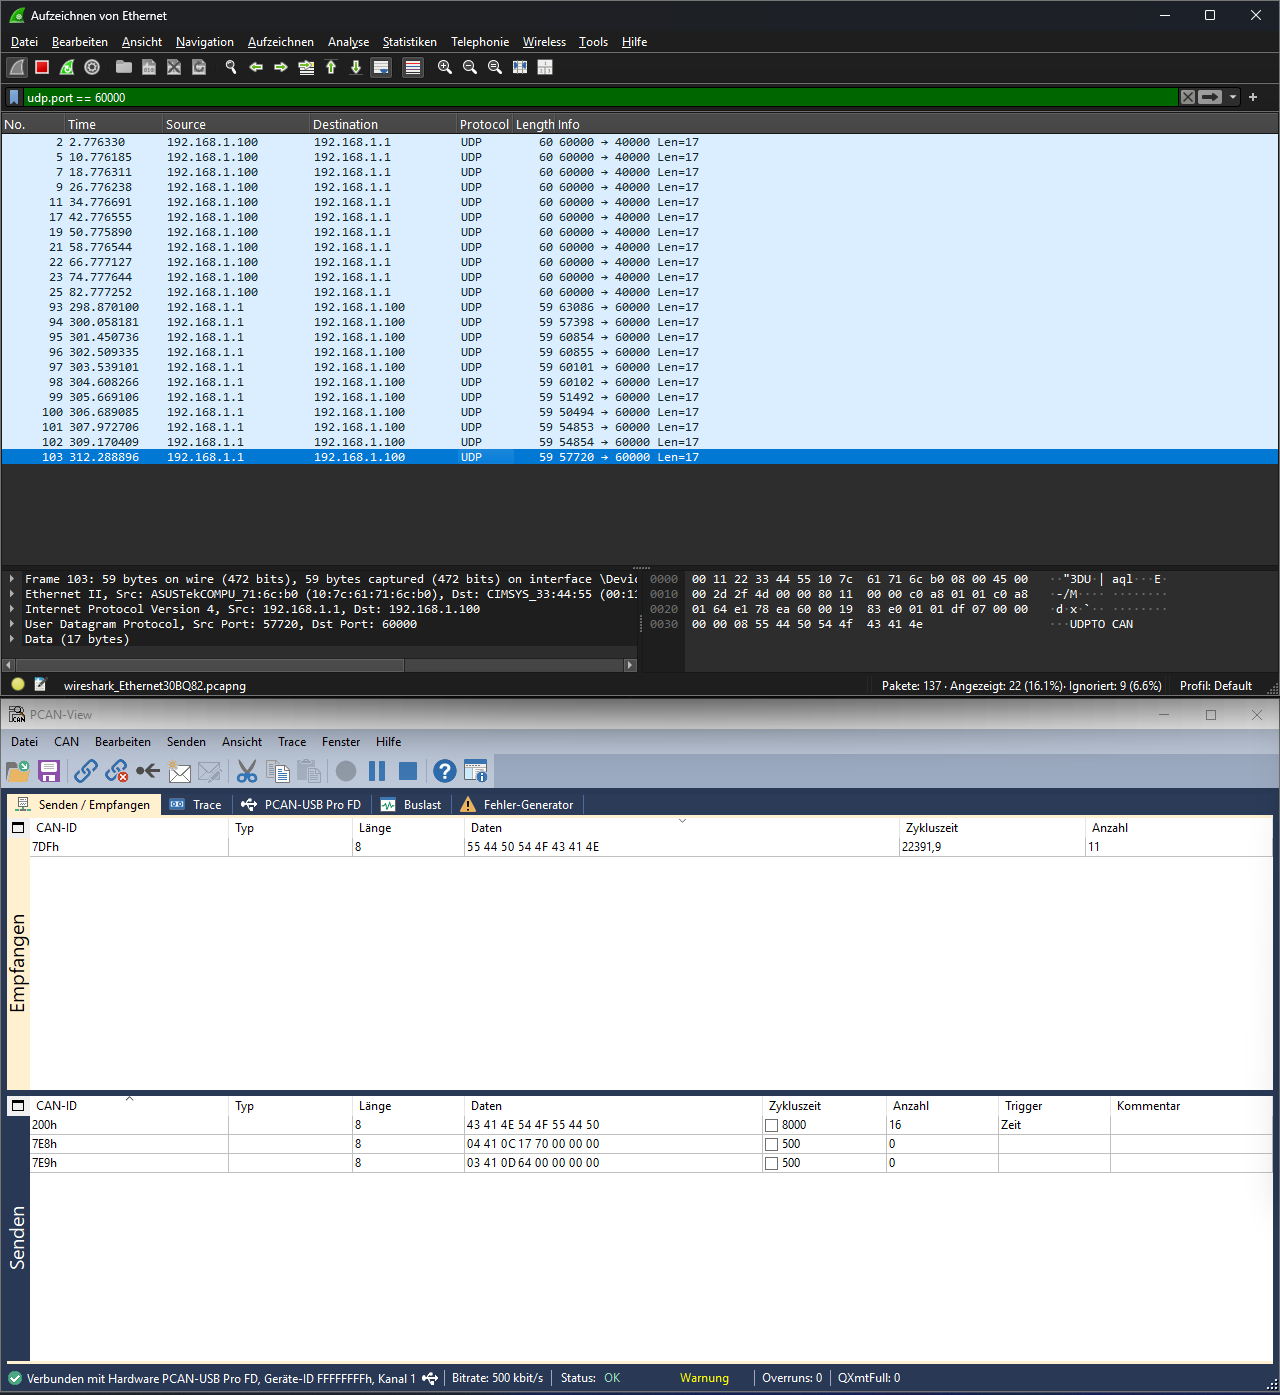
\includegraphics[width=0.8\textwidth]{figures/pictures/ethtocan.png}
    \caption{Ethernet to Can}
    \label{fig:results}
\end{figure}
In Figure 5, Wireshark records multiple UDP packets originating from a PC (192.168.1.1) and addressed to the microcontroller at 192.168.1.100 on port 60000. Each UDP payload is exactly 17 bytes long, conforming to the defined CAN message encapsulation format. The payload contains a recognizable ASCII sequence “UDPTOCAN,” which serves as a test marker. Simultaneously, the lower window (PCAN-View) shows that the CAN message with ID \verb|0x7DF| and the correct payload bytes has been successfully received and decoded by a connected CAN interface. This demonstrates that the embedded function \verb|forwardEthernetToCan()| correctly extracted and transmitted the CAN message based on the incoming UDP frame.
\begin{figure}[h]
    \centering
     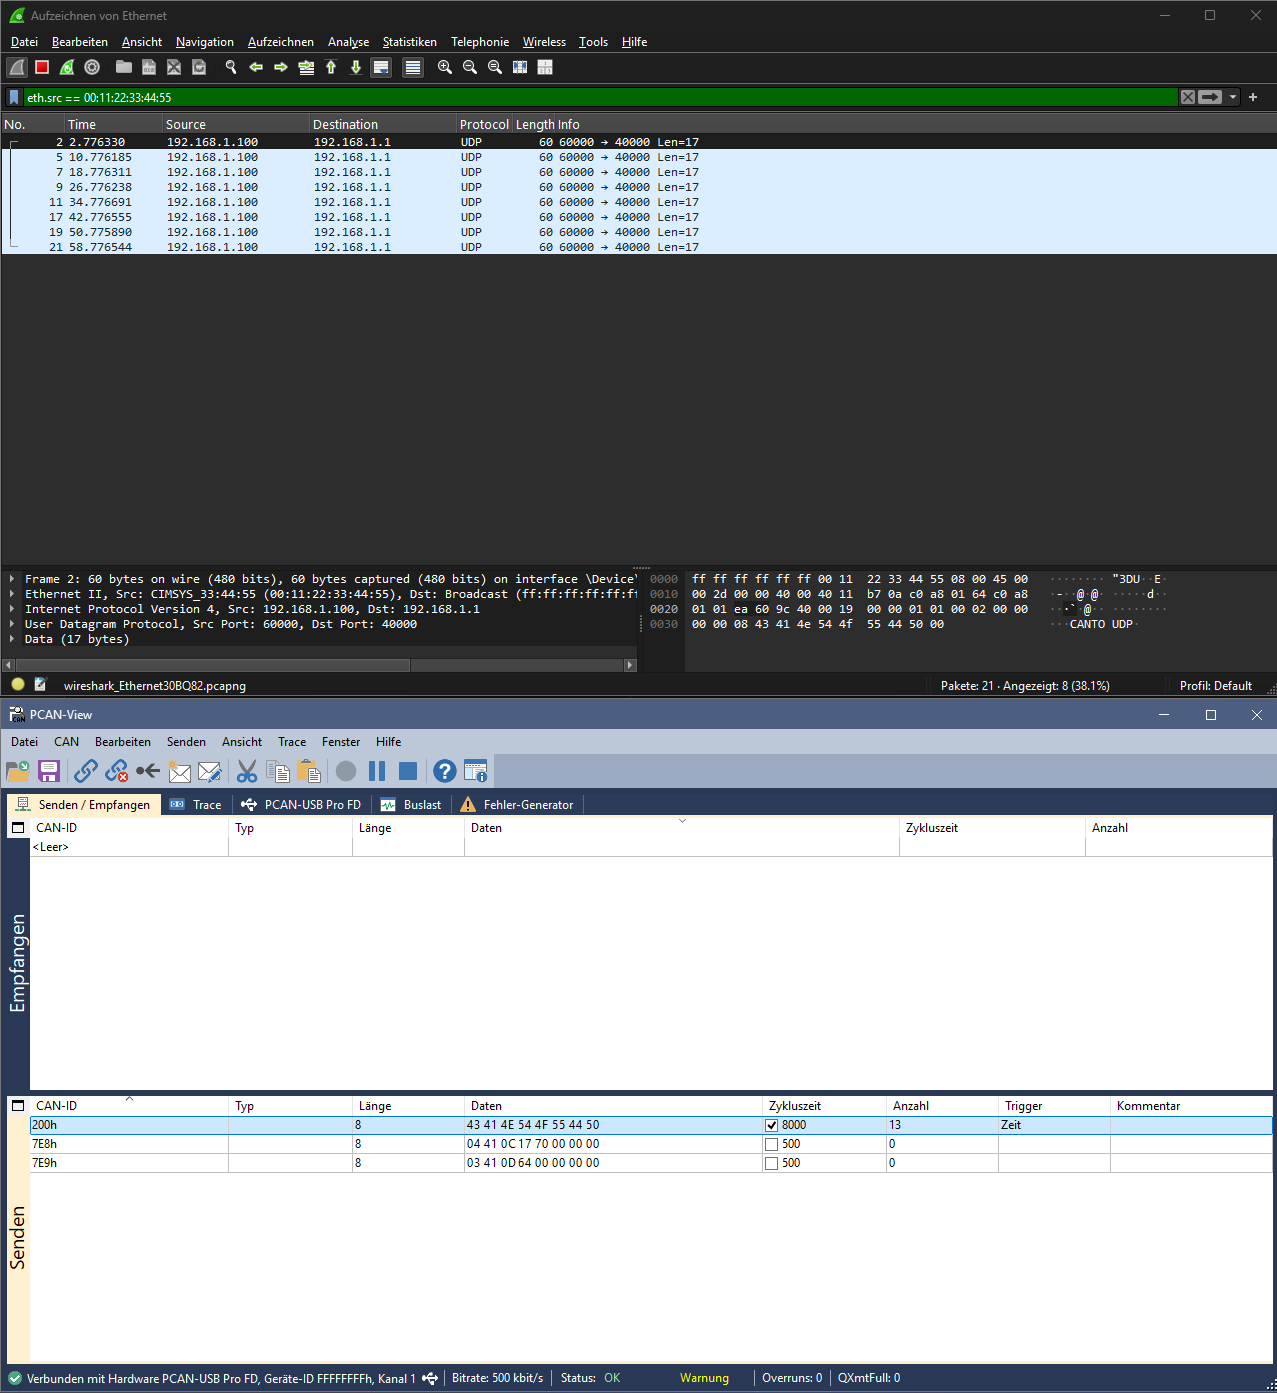
\includegraphics[width=0.8\textwidth]{figures/pictures/cantoeth.png}
    \caption{Can to Ethernet}
    \label{fig:results}
\end{figure}\\
Figure 6 shows the reverse communication path. Here, the CAN message with ID \verb|0x200| and data payload corresponding to the ASCII string “CANTOUDP” is transmitted from the CAN bus. Wireshark captures its Ethernet encapsulation, showing correct transmission from the microcontroller to a broadcast destination (MAC: FF:FF:FF:FF:FF:FF) on UDP port 40000. The embedded function \verb|forwardCanToEthernet()| has successfully serialized the CAN frame into a valid UDP packet and injected it into the Ethernet stack.\\\\
Together, these bidirectional traces confirm that both gateway directions—Ethernet to CAN and CAN to Ethernet—function as intended. The protocol is correctly formed, hardware peripherals are synchronized, and application-layer behavior is predictable and reliable. This validation confirms that the goals of the project were achieved and a fully operational CAN-Ethernet gateway with UDP support was realized on the Infineon TriCore platform.


\centering
\begin{sequencediagram}
    \newthread{runEthernetLogic}{runEthernetLogic}    
    \newinst{eth}{sendEthernetPacket}
    \newinst{dma}{getReceiveBuffer}
    \newinst{phy}{Phy\_Pef7071}

    \begin{call}{runEthernetLogic}{link()}{phy}{}
    \end{call}

    \begin{sdblock}{if g\_sendAliveMessage}{ }
        \begin{call}{runEthernetLogic}{"i am alive"}{eth}{}
        \end{call}
    \end{sdblock}

    \begin{call}{runEthernetLogic}{ }{dma}{rx\_data}
        \begin{sdblock}{if rx\_data}{ }
            \begin{call}{dma}{freeReceiveBuffer()}{dma}{}
            \end{call}
        \end{sdblock}
    \end{call}
\end{sequencediagram}
\caption{Ethernet Rx/Tx Logic}

\begin{figure}{!h}
\centering
\begin{sequencediagram}
    \newthread{app}{Application}
    \newinst{tx}{transmitCanMessage}
    \newinst{rx}{receiveCanMessage}
    \newinst{hw}{MultiCAN HW}

    \begin{call}{app}{message}{tx}{status}
        \begin{sdblock}{while busy}{ }
             \begin{call}{tx}{sendMessage()}{hw}{}
             \end{call}
        \end{sdblock}
    \end{call}

    \begin{call}{app}{ }{rx}{status, msg}
        \begin{call}{rx}{readMessage()}{hw}{}
        \end{call}
    \end{call}
\end{sequencediagram}
\caption{UML Diagramm: CAN Rx/Tx Logic}
\label{uml:can}
\end{figure}
\begin{figure}
\centering
\begin{sequencediagram}
    % Define lifelines
    \newthread{fwd_can_eth}{forwardCanToEthernet}
    \newinst{multican}{MultiCAN Driver}
    \newinst{eth}{Ethernet Driver}

    % Sequence of calls with corrected syntax
    \begin{call}{fwd_can_eth}{isRxPending}{multican}{isPending}\end{call}

    \begin{sdblock}{alt}{[isPending is TRUE]}
    
        \begin{call}{fwd_can_eth}{getPointer}{multican}{}\end{call}
        
        \begin{call}{fwd_can_eth}{readMessage}{multican}{rxMsg}\end{call}
        
        \begin{callself}{fwd_can_eth}{Construct UDP Payload from CAN data}{}\end{callself}

        \begin{call}{fwd_can_eth}{sendEthernetPacket}{eth}{}\end{call}
        
        \begin{call}{fwd_can_eth}{clearRxPending}{multican}{}\end{call}
        
    \end{sdblock}

\end{sequencediagram}
\caption{CAN to Ethernet Message Forwarding}
\end{figure}
\begin{figure}
\centering
\begin{sequencediagram}
    % Define lifelines
    \newthread{fwd_eth_can}{forwardEthernetToCan}
    \newinst{eth_driver}{Ethernet Driver}
    \newinst{can_driver}{MultiCAN Driver}

    % Sequence of calls with corrected syntax
    \begin{call}{fwd_eth_can}{receiveEthernetPacket}{eth_driver}{payloadLen}\end{call}

    \begin{sdblock}{alt}{[payloadLen > 0]}
        
        %\node[note, text width=4cm] (validation_note) [right=of fwd_eth_can] 
        %    {Internal Validation & Parsing:
        %    \begin{itemize}
        %        \item Check packet header and DLC
        %        \item Extract CAN ID, Data, frame type
        %    \end{itemize}
        %};
        
        \begin{sdblock}{alt}{[frame is DATA and ID is STANDARD]}
            
            \begin{callself}{fwd_eth_can}{IfxMultican\_Message\_init}{canMsg}\end{callself}

            % The call to the driver, which contains the loop
            \begin{call}{fwd_eth_can}{transmitCanMessage}{can_driver}{}
                
                \begin{sdblock}{loop}{[while TX buffer is busy]}
                    % The internal driver call
                    \begin{call}{can_driver}{sendMessage}{can_driver}{status}\end{call}
                \end{sdblock}
                
            \end{call}

        \end{sdblock}
    \end{sdblock}
\end{sequencediagram}
\\
\caption{UML Diagramm: Ethernet to CAN Message Forwarding}
\label{uml:ethtocan}
\end{figure}